\section{HIỆN THỰC HỆ THỐNG}

\subsection{Kiến trúc triển khai}
\hspace{1cm}
Toàn bộ hệ thống được đóng gói bằng \textbf{Docker Compose}, khai báo trong tệp
\texttt{infra/docker-compose.yml}, gồm các thành phần sau chạy độc lập và giao tiếp qua mạng
nội bộ container:

\begin{table}[H]
\centering
\caption{Thành phần dịch vụ trong hệ thống}
\begin{tabular}{@{}>{\raggedright\arraybackslash}p{3.9cm}>{\raggedright\arraybackslash}p{2.9cm}>{\raggedright\arraybackslash}p{7.2cm}@{}}
\toprule
\textbf{Dịch vụ} & \textbf{Công nghệ} & \textbf{Vai trò} \\
\midrule
\texttt{db} & PostgreSQL & Lưu trữ staging + kho dữ liệu (schema \texttt{dw}). \\
\texttt{airflow-\allowbreak webserver}, \newline \texttt{airflow-\allowbreak scheduler} & Apache Airflow & Điều phối và giám
sát các DAG ETL/DSS batch. \\
\texttt{dss} & FastAPI (Python, scikit-learn) & Model service: huấn luyện, chấm điểm,
what-if và dự đoán cho đơn tự nhập với hai mô hình rủi ro (giao trễ, đánh giá thấp). \\
\texttt{backend-api} & FastAPI (Python) & Backend-for-Frontend (BFF): tổng hợp dữ liệu từ
OLAP view và DSS service thành API cho frontend. \\
\texttt{frontend} & React + Vite + TypeScript & Một ứng dụng tại http://localhost:5173, gồm bốn màn hình (giao diện tiếng Anh): Manager Dashboard, Ops Console, Campaign, Risk Predictor. \\
\bottomrule
\end{tabular}
\end{table}

\subsection{Backend API (BFF)}
\hspace{1cm}
\texttt{backend-api} đóng vai trò \textit{Backend-for-Frontend}, tách biệt hai mối quan tâm:
(1) truy vấn thống kê thuần túy thực hiện trực tiếp trên các OLAP view của kho dữ liệu; (2)
truy vấn liên quan đến mô hình DSS được chuyển tiếp (proxy) sang \texttt{dss} service. Các
module chính trong \texttt{backend-api/app/modules/}:

\begin{itemize}
    \item \texttt{dashboard.py} -- KPI tổng (doanh thu, số đơn, AOV tính trên
          \texttt{FACT\_ORDER\_ITEM}; tỷ lệ giao trễ và điểm đánh giá trung bình tính theo đơn trên
          \texttt{FACT\_ORDER\_FULFILLMENT}, cùng cách tính với phần giao hàng và mô hình DSS), xu hướng doanh thu có lọc theo năm/ngành/vùng,
          top sản phẩm bán chạy/chậm cho Manager Dashboard (đọc từ
          \texttt{mv\_revenue\_by\_\allowbreak month\_category}, \texttt{mv\_top\_products}).
    \item \texttt{dashboard.py} (tiếp) -- hiệu suất giao hàng theo tháng
          (\texttt{/dashboard/\allowbreak delivery-trend}), tuyến giao trễ nhiều nhất
          (\texttt{/dashboard/\allowbreak delivery-routes}), đọc từ \texttt{mv\_delivery\_\allowbreak performance}; điểm
          đánh giá theo mức trễ (\texttt{/dashboard/\allowbreak review-by-delay}).
    \item \texttt{risk.py} -- proxy sang \texttt{dss}: thống kê theo mức rủi ro
          (\texttt{GET /risk/\{model\}/summary}), danh sách đơn rủi ro
          (\texttt{GET /risk/\{model\}/orders}), chỉ số và feature importance của mô hình (dùng cho
          báo cáo, giao diện không hiển thị),
          what-if (\texttt{POST /risk/\{model\}/what-if}), dự đoán cho đơn tự nhập
          (\texttt{POST /risk/\{model\}/predict}, kèm \texttt{GET /risk/predict/options} và
          \texttt{GET /risk/predict/distance} để form nạp danh sách bang, ngành và tự điền
          khoảng cách).
    \item \texttt{campaigns.py} -- thêm, sửa, xóa chiến dịch chăm sóc
          (\texttt{GET/POST /campaigns}, \texttt{PUT/DELETE /campaigns/\{code\}});
          gán/xem/xóa tệp khách hàng chăm sóc:
          khách của các đơn có rủi ro đánh giá thấp $\geq$ ngưỡng do Ops chọn
          (\texttt{POST /campaigns/\{code\}/targets?min\_risk=}, bảng \texttt{dw.campaign\_target}).
\end{itemize}

Kết nối cơ sở dữ liệu được quản lý tập trung tại \texttt{app/db.py}, sử dụng SQLAlchemy engine
với connection pooling. Các module gọi sang \texttt{dss} chỉ chuyển tiếp (proxy) yêu cầu qua một
\texttt{httpx} client dùng chung, giữ nguyên mã lỗi 4xx và thông báo của \texttt{dss} (ví dụ
400 khi bang không có trong dữ liệu train, 409 khi mô hình chưa được huấn luyện).

\subsection{Frontend}
\hspace{1cm}
Frontend là \textbf{một} ứng dụng \textbf{React + TypeScript + Vite} duy nhất
(\texttt{frontend/}), chạy ở một cổng 5173. Mỗi nhóm người dùng ở Mục 2.2 có một màn hình
riêng, chọn bằng route dạng hash (\texttt{\#/manager}, \texttt{\#/ops}, \texttt{\#/campaigns}, \texttt{\#/predict}) khai báo trong
\texttt{src/App.tsx}. Bốn màn hình được chọn qua một thanh tab nằm ngang ở đầu trang, tab đang mở được
tô nổi. Toàn bộ giao diện hiển thị bằng \textbf{tiếng Anh}; tiền (BRL) và số theo định dạng tiếng Anh, ví dụ
\texttt{R\$13,494,401}, nhãn trục rút gọn \texttt{R\$1.2M}, số đếm \texttt{98,199}. Mã bang và mã ngành
vẫn được gửi nguyên giá trị gốc khi gọi API, chỉ đổi cách hiển thị (tên đủ 27 bang, \texttt{cool\_stuff}
$\to$ \textit{Cool Stuff}). Biểu đồ vẽ bằng thư viện \textbf{Recharts}, biểu tượng dùng
\textbf{lucide-react}. Mọi lời gọi API tập trung trong \texttt{src/api.ts}. Các thành phần giao diện dùng chung
(tiêu đề, bảng sắp xếp được, trạng thái đang tải/lỗi/trống, ô chọn số dòng, nút tải tệp) nằm trong
\texttt{src/components/}, các hàm định dạng nằm trong \texttt{src/utils/}, CSS nằm trong \texttt{src/styles.css}:

\begin{itemize}
    \item \textbf{Manager Dashboard} (\texttt{src/pages/ManagerDashboard.tsx}): thẻ KPI, biểu
          đồ doanh thu theo tháng và theo bang có bộ lọc năm/ngành/vùng (slice/dice) và nút
          \textit{Export report} xuất doanh thu theo bộ lọc ra CSV; tỷ lệ giao trễ và tỷ lệ đánh
          giá thấp theo tháng, tỷ lệ đánh giá thấp theo mức trễ, 10 tuyến giao trễ nhiều nhất và
          10 sản phẩm có doanh thu thấp nhất.
    \item \textbf{Ops Console} (\texttt{src/pages/OpsConsole.tsx}): danh sách đơn có rủi ro
          giao trễ (các đơn đang vận chuyển, còn can thiệp được) và đơn vừa giao có
          rủi ro đánh giá thấp, lọc theo mức High/Medium/Low hoặc tất cả, chọn số dòng hiển thị
          trên tổng số đơn, tải các dòng đang hiển thị về tệp \texttt{.csv} hoặc \texttt{.xlsx};
          đơn giao trễ có nút \textit{Simulate action} mở bảng mô phỏng ngay dưới dòng đó để thử
          dời ngày hẹn giao thêm $N$ ngày và so sánh rủi ro trước/sau (không lưu thay đổi vào đơn);
          công cụ ``gắn các khách hàng có rủi ro review thấp $\geq$ ngưỡng vào chiến dịch đã
          chọn'' (danh sách lấy từ màn hình Campaign). Chất lượng mô hình (chỉ số, đối chiếu mức
          rủi ro với kết quả thật, feature importance) không hiển thị trên giao diện vận hành mà
          được trình bày trong báo cáo (Mục~\ref{sec:model-results}).
    \item \textbf{Campaign} (\texttt{src/pages/CampaignManager.tsx}): danh sách chiến dịch chăm
          sóc hiển thị trước; nút \textit{Create campaign} mở form tạo ngay trên trang; sửa tên, mô
          tả và xoá ngay trong bảng; nút \textit{Details} hiện mô tả cùng danh sách khách đã gắn
          (xếp theo rủi ro giảm dần), số khách và rủi ro trung bình. Cả hai danh sách đều có ô chọn
          số dòng và nút tải tệp \texttt{.csv} hoặc \texttt{.xlsx}.
    \item \textbf{Risk Predictor} (\texttt{src/pages/RiskPredictor.tsx}): công cụ chấm điểm
          cho một đơn do người dùng tự nhập (Mục~5.6). Phần \textit{Order details} dùng chung cho
          hai mô hình: bang người bán, bang khách, khoảng cách (tự điền ngay khi chọn hai bang,
          sửa được), ngành hàng, ngày mua, ngày hẹn giao. Mỗi mô hình có thêm ô riêng: ngày bàn
          giao vận chuyển và hạn bàn giao (mô hình giao trễ), ngày giao tới khách (mô hình đánh
          giá thấp). Kết quả gồm phần trăm rủi ro, mức High/Medium/Low trên thanh có vạch ngưỡng,
          tỷ lệ lịch sử của tuyến và bảng \textit{Model inputs} liệt kê giá trị mô hình đã dùng kèm
          nguồn. Đổi bất kỳ thông tin đơn nào sau khi dự đoán thì kết quả cũ bị xoá để tránh đọc nhầm.
\end{itemize}

Hình~\ref{fig:ui-manager}--\ref{fig:ui-predict} là ảnh chụp bốn màn hình khi chạy với dữ liệu thật.

\begin{figure}[H]
\centering
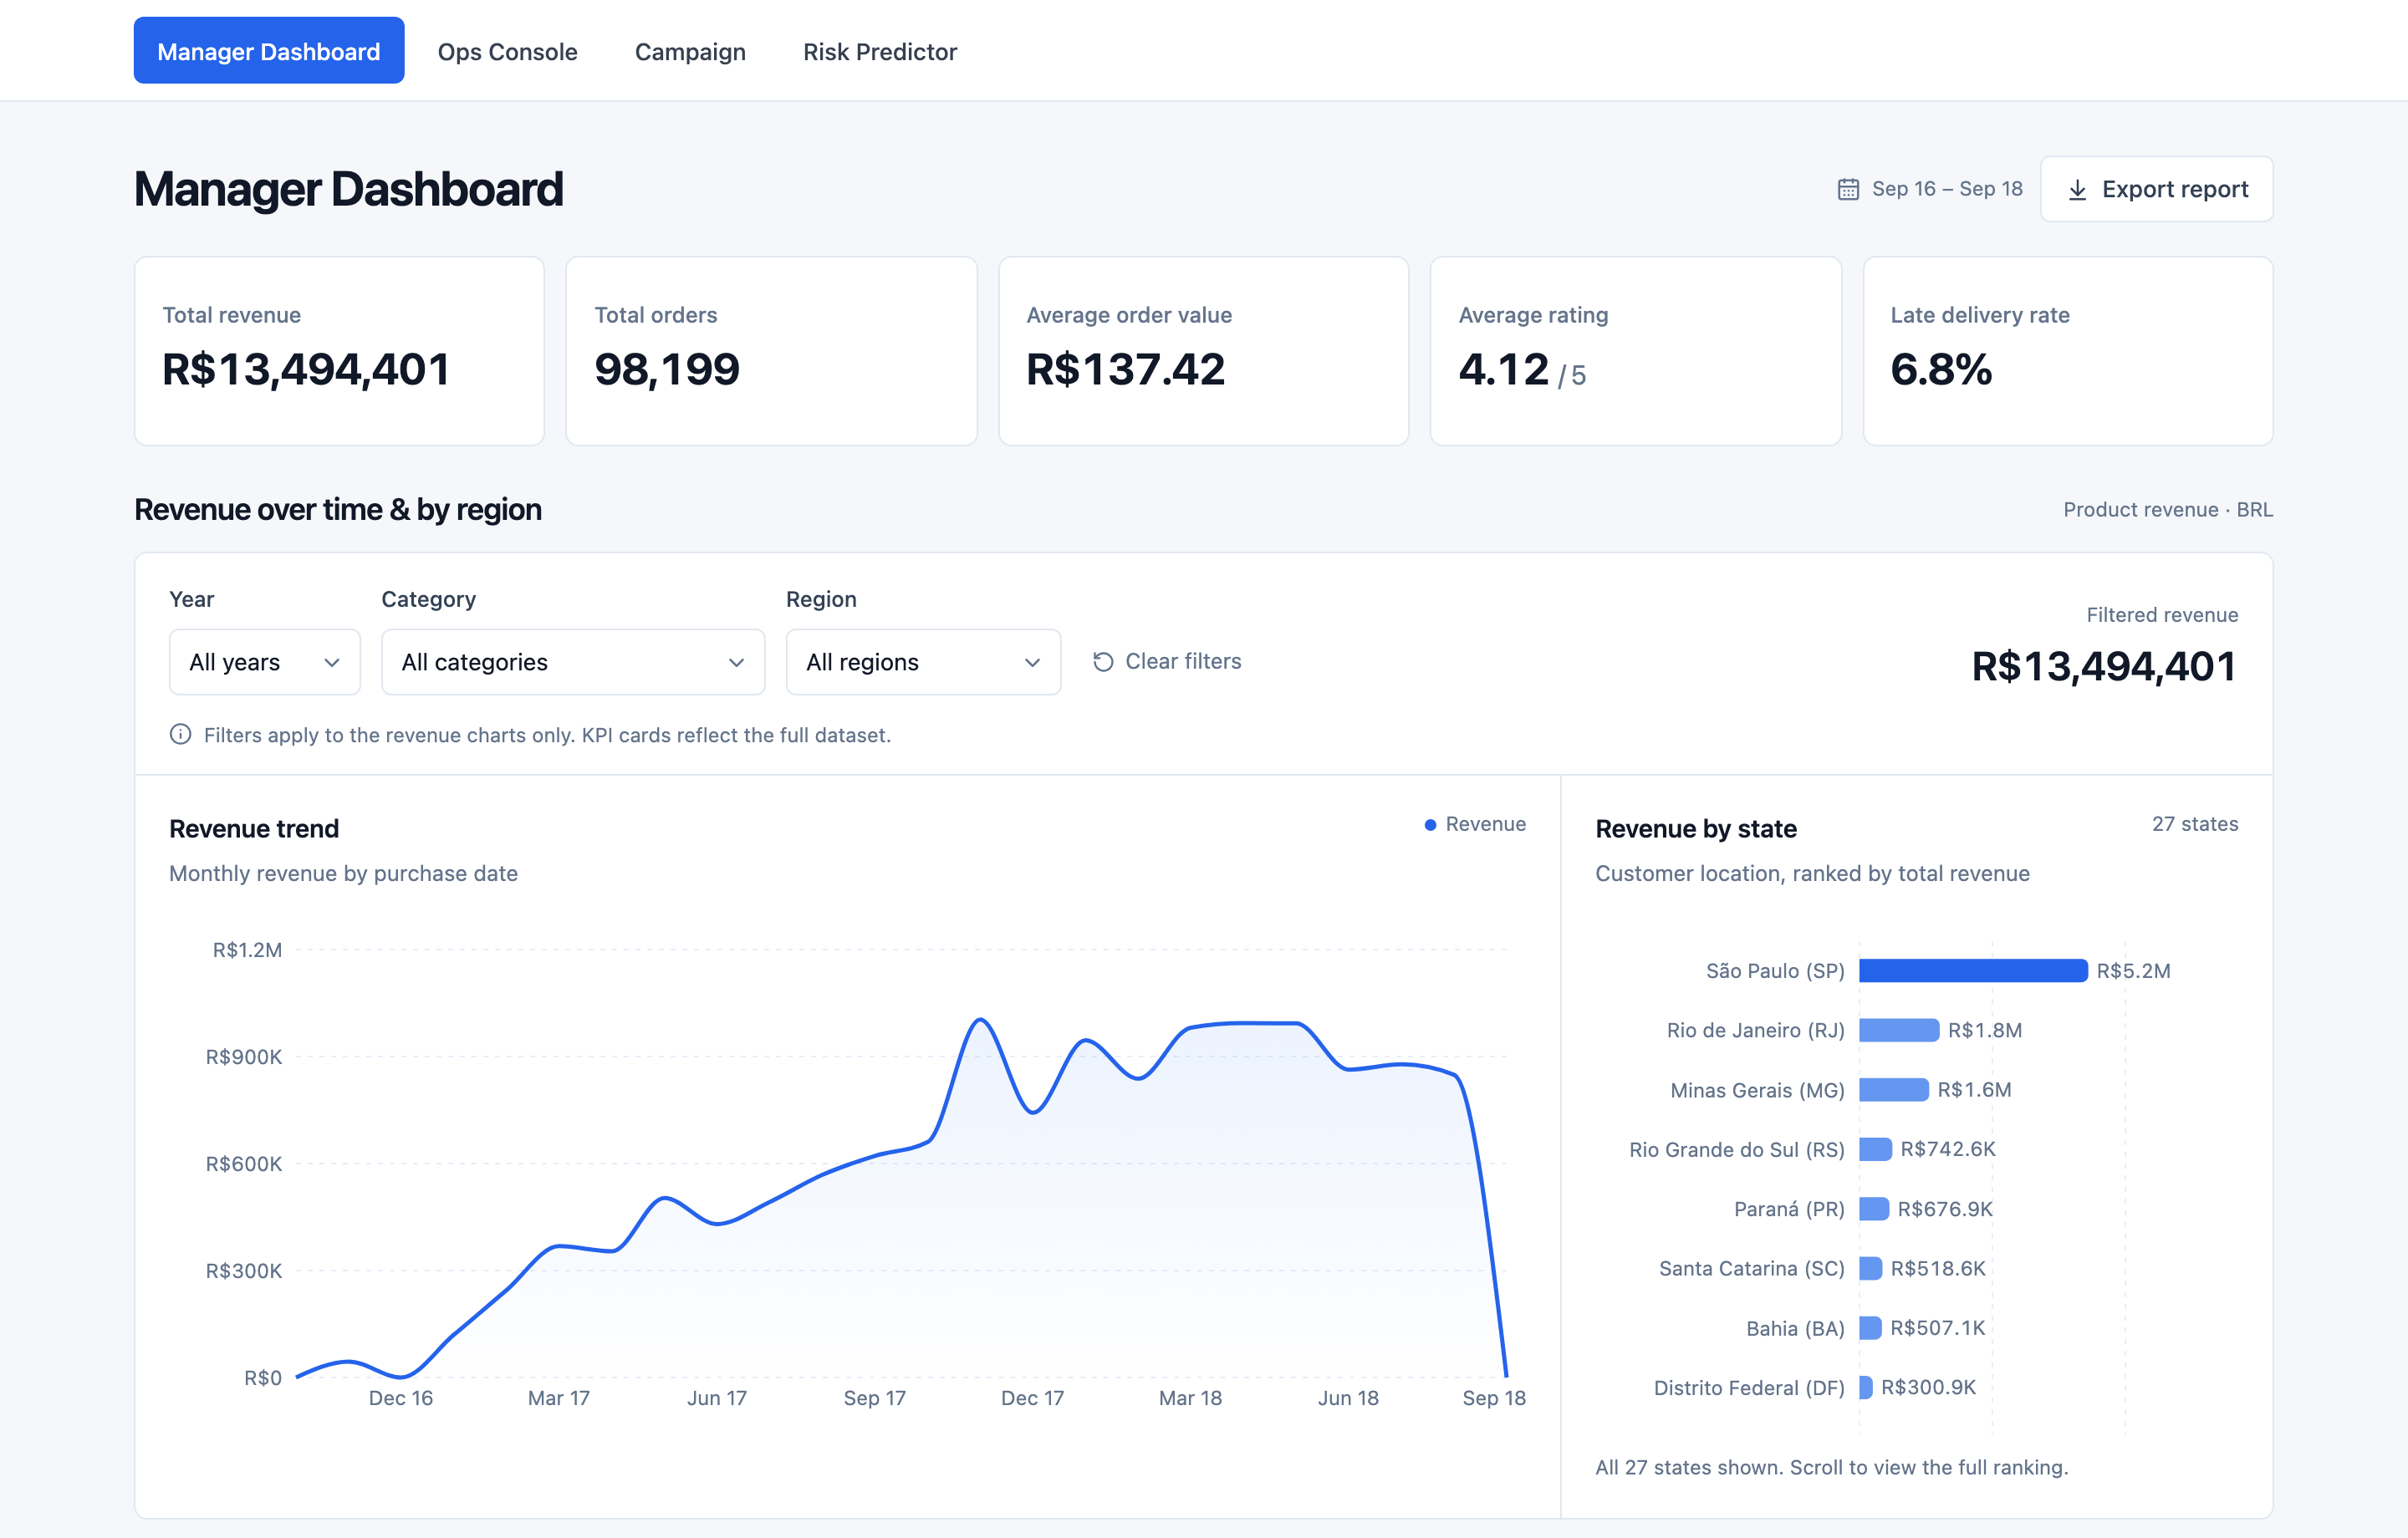
\includegraphics[width=0.85\textwidth]{Picture/ui_manager_overview.png}
\caption{Manager Dashboard: thanh tab trên cùng, thẻ KPI, doanh thu theo tháng và theo bang với bộ lọc năm/ngành/vùng}
\label{fig:ui-manager}
\end{figure}

\begin{figure}[H]
\centering
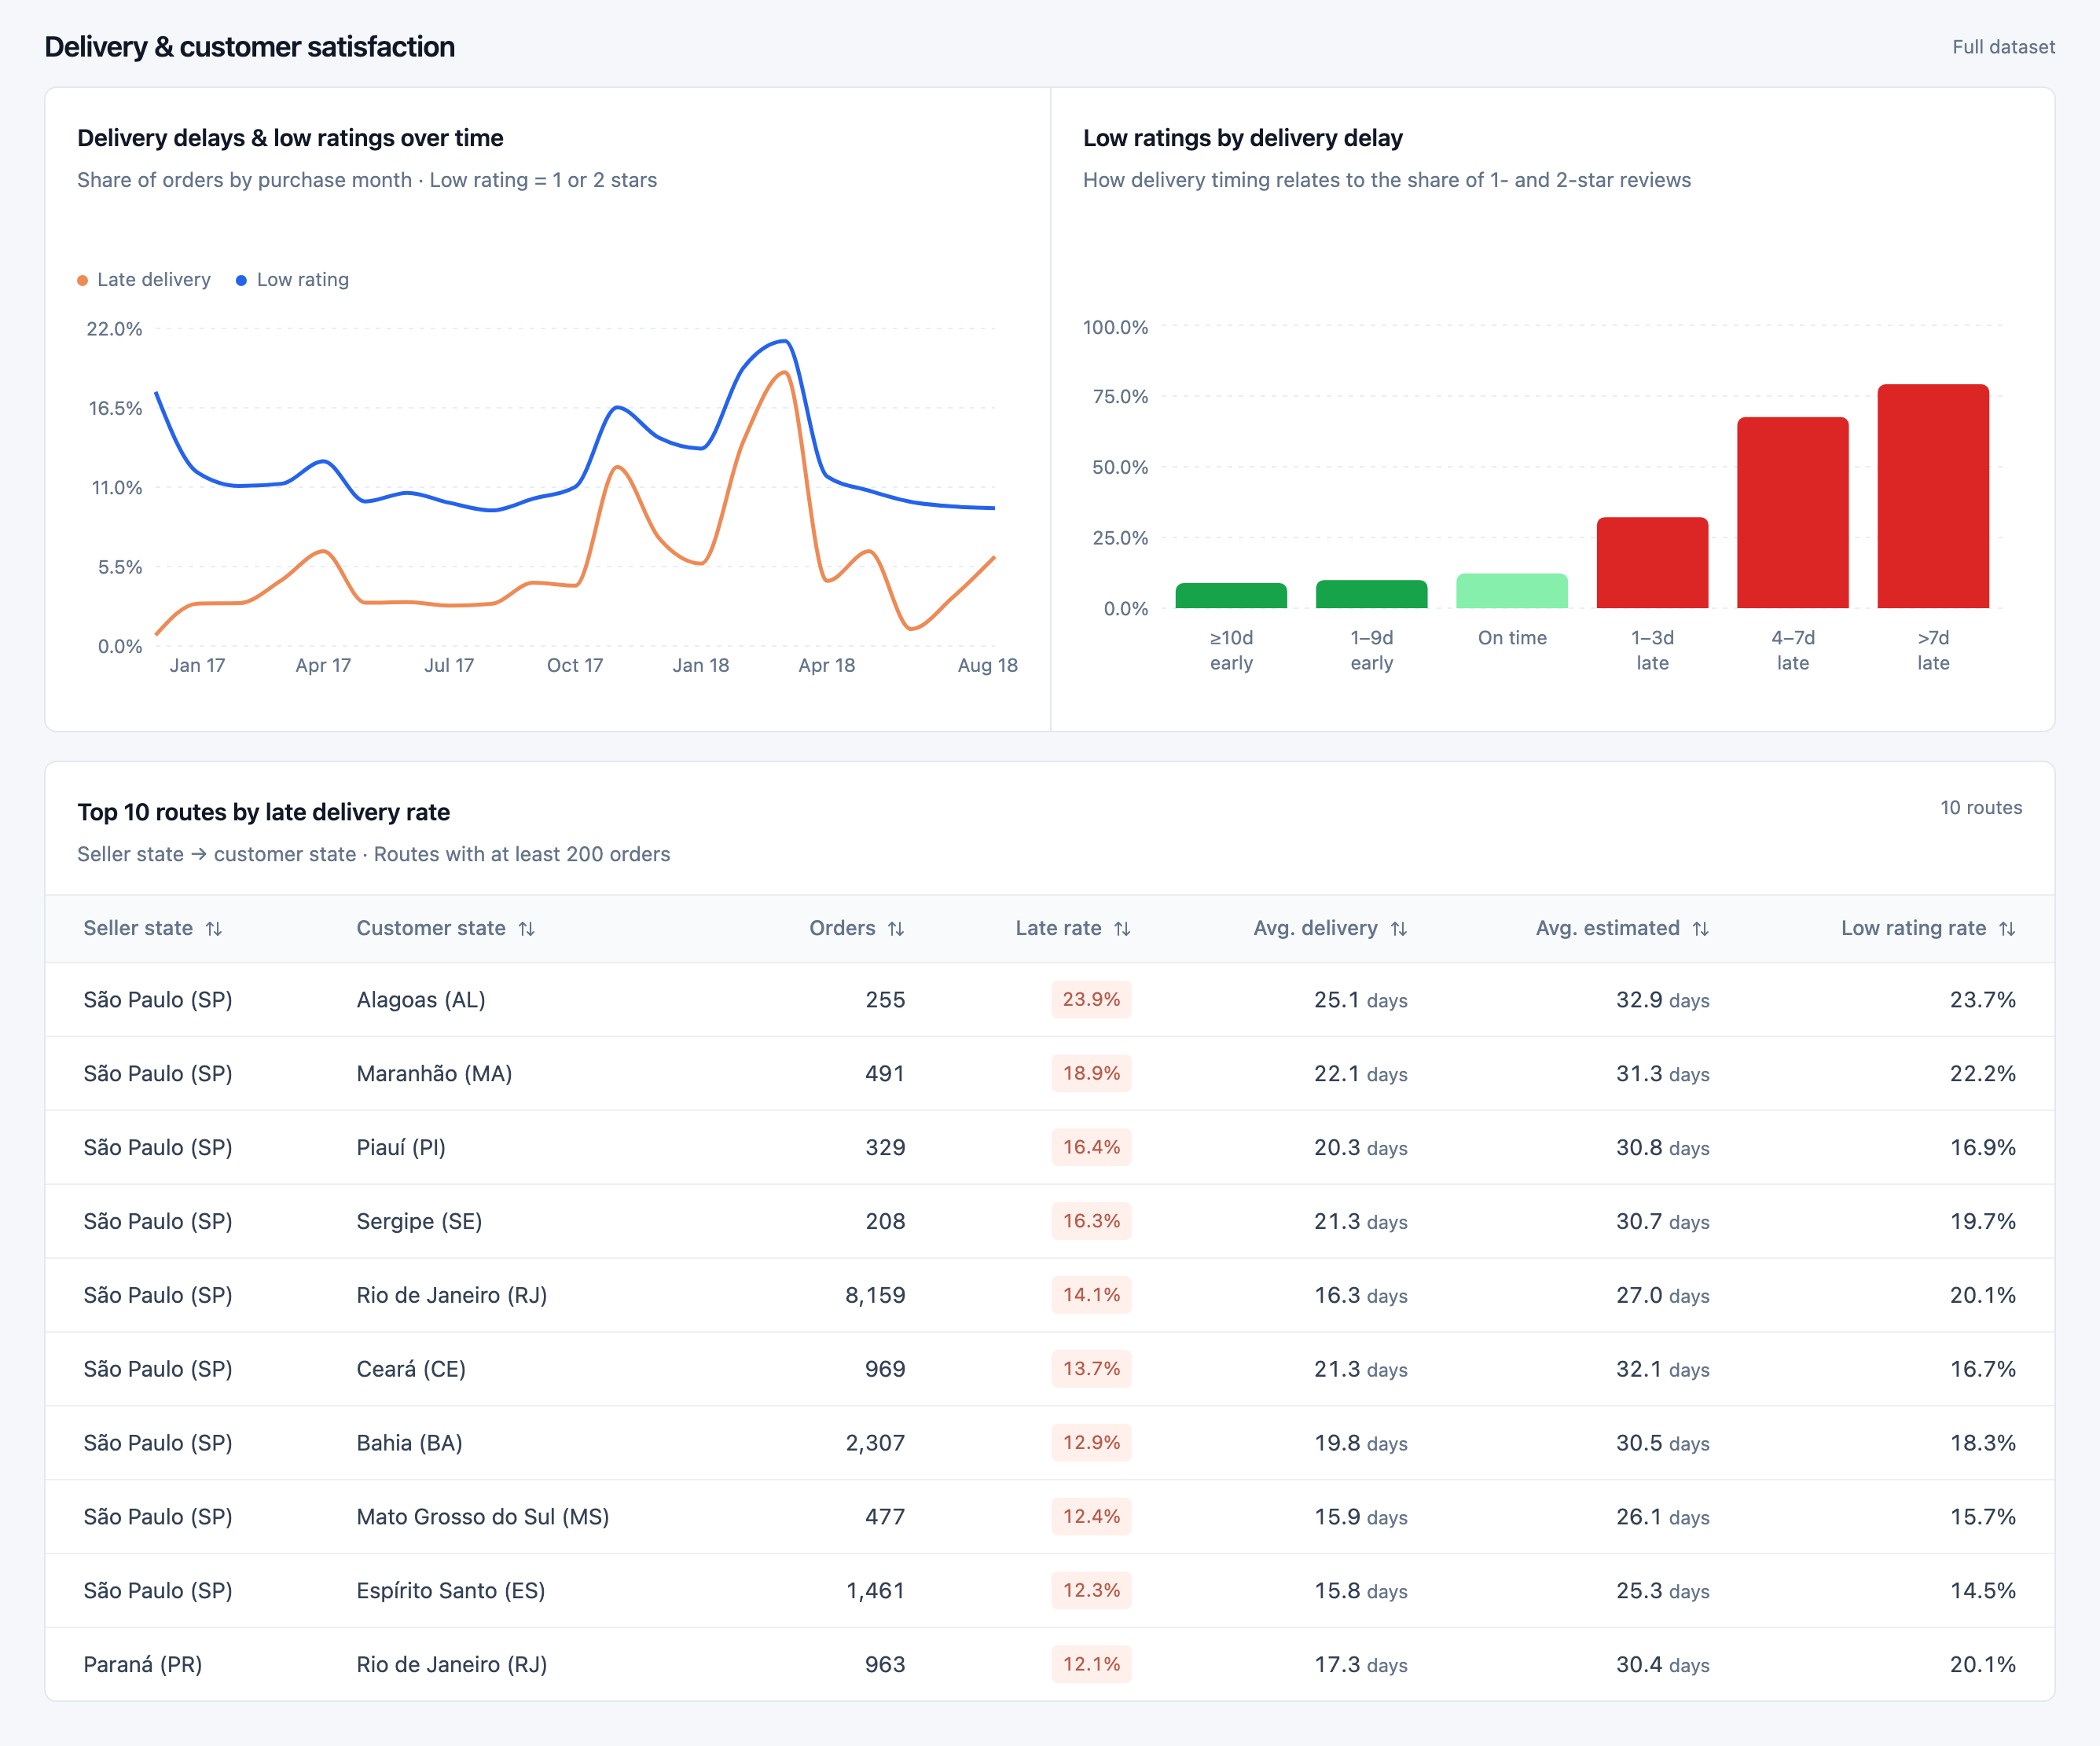
\includegraphics[width=0.85\textwidth]{Picture/ui_manager_delivery.png}
\caption{Manager Dashboard: phần giao hàng và mức độ hài lòng}
\label{fig:ui-delivery}
\end{figure}

\begin{figure}[H]
\centering
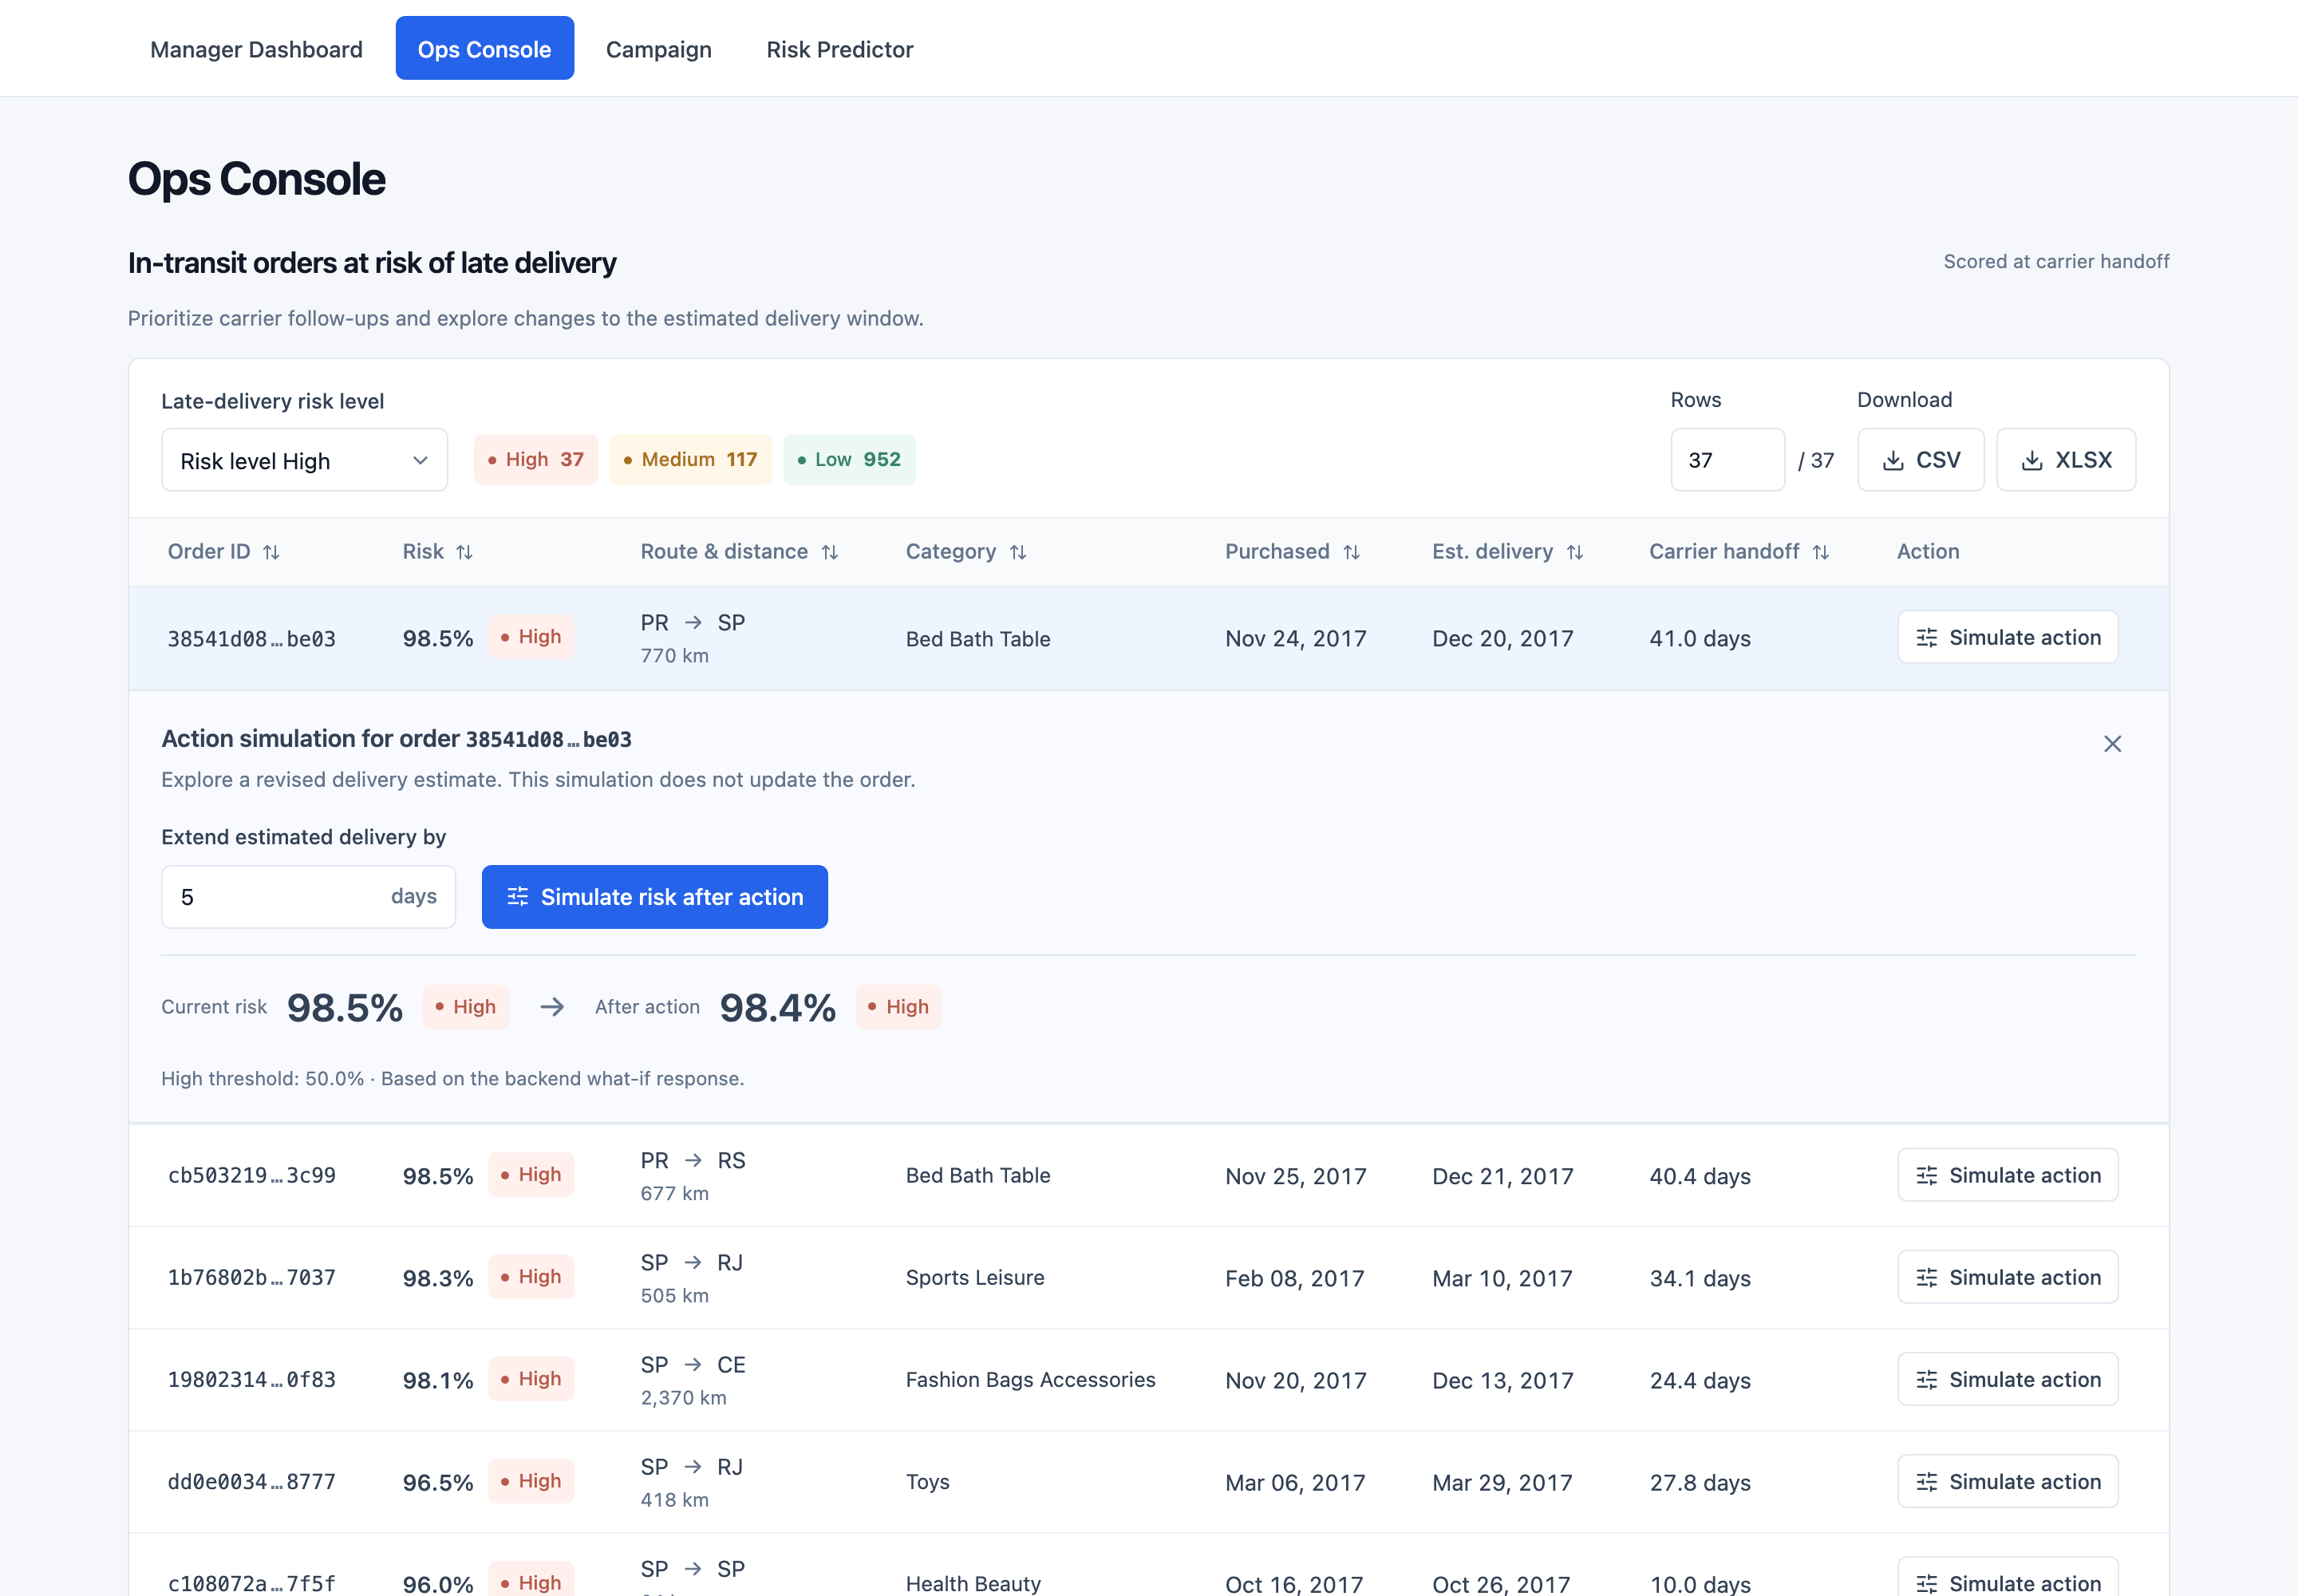
\includegraphics[width=0.85\textwidth]{Picture/ui_ops_late.png}
\caption{Ops Console: danh sách đơn đang vận chuyển có rủi ro giao trễ mức High kèm số đơn theo từng mức, ô chọn số dòng, nút tải CSV/XLSX và nút Simulate action}
\label{fig:ui-ops-late}
\end{figure}

\begin{figure}[H]
\centering
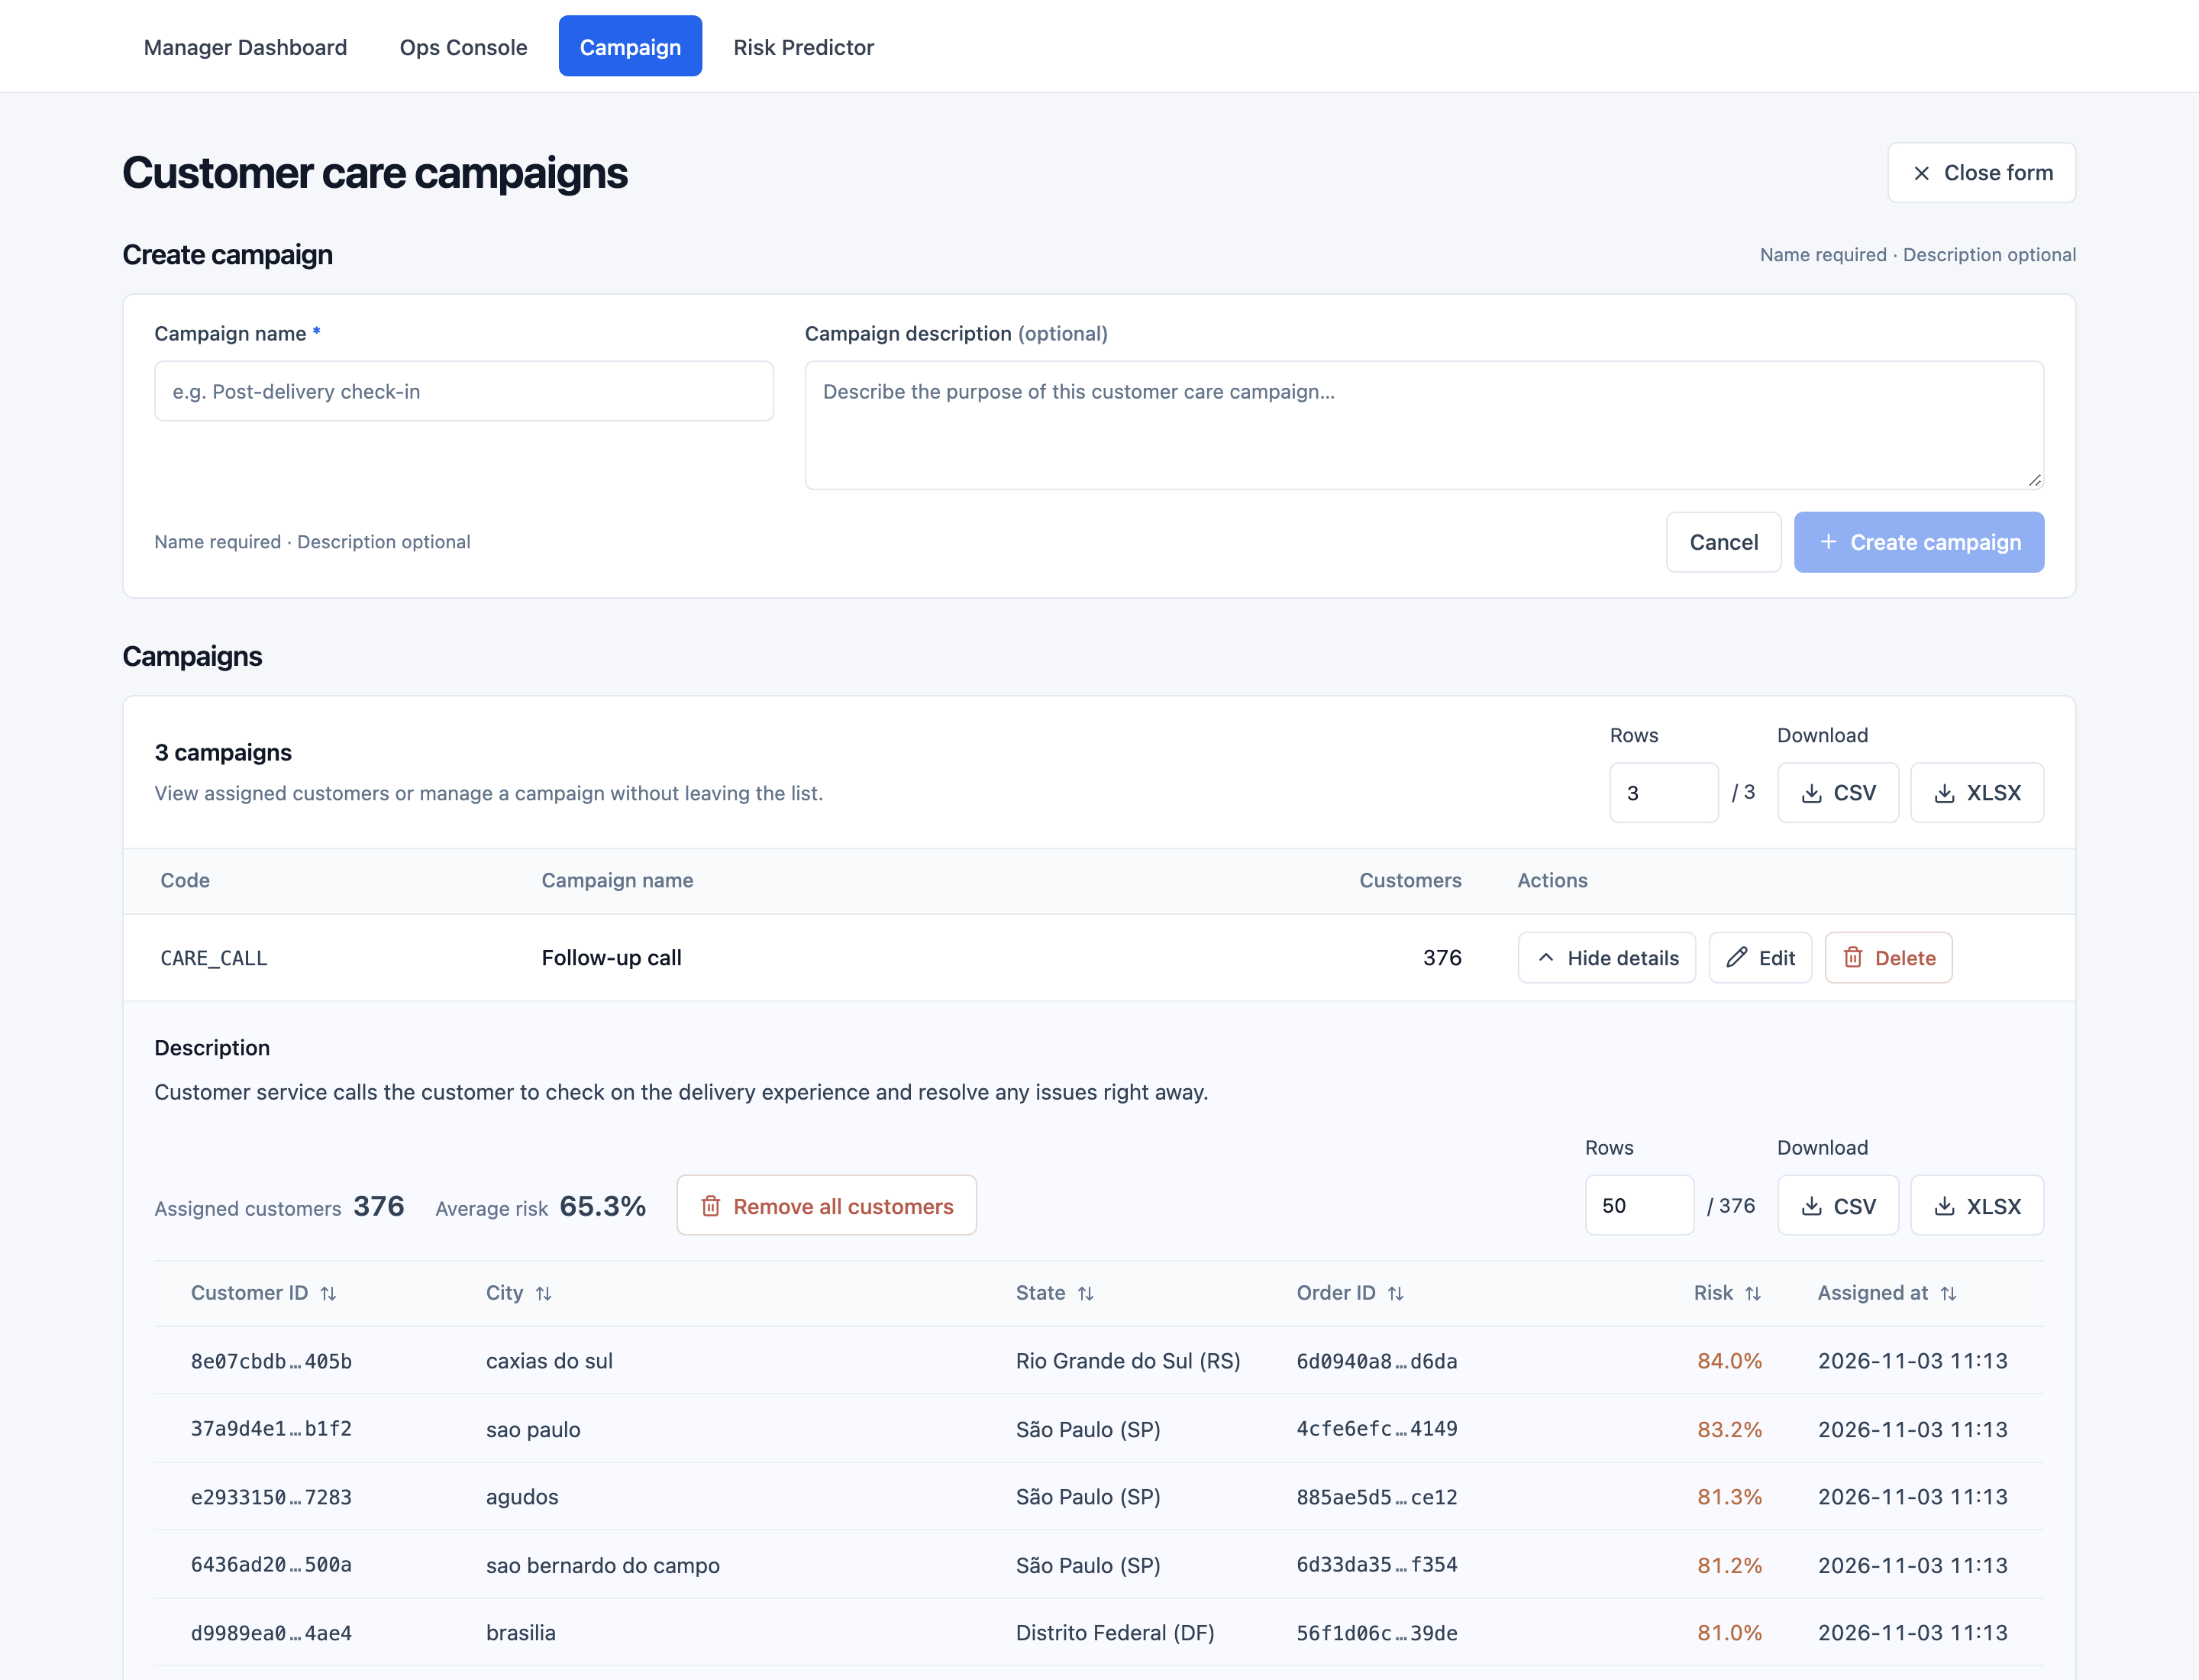
\includegraphics[width=0.85\textwidth]{Picture/ui_campaign.png}
\caption{Màn hình Campaign: danh sách chiến dịch, form thêm mới, phần chi tiết gồm mô tả và khách đã gắn}
\label{fig:ui-campaign}
\end{figure}

\begin{figure}[H]
\centering
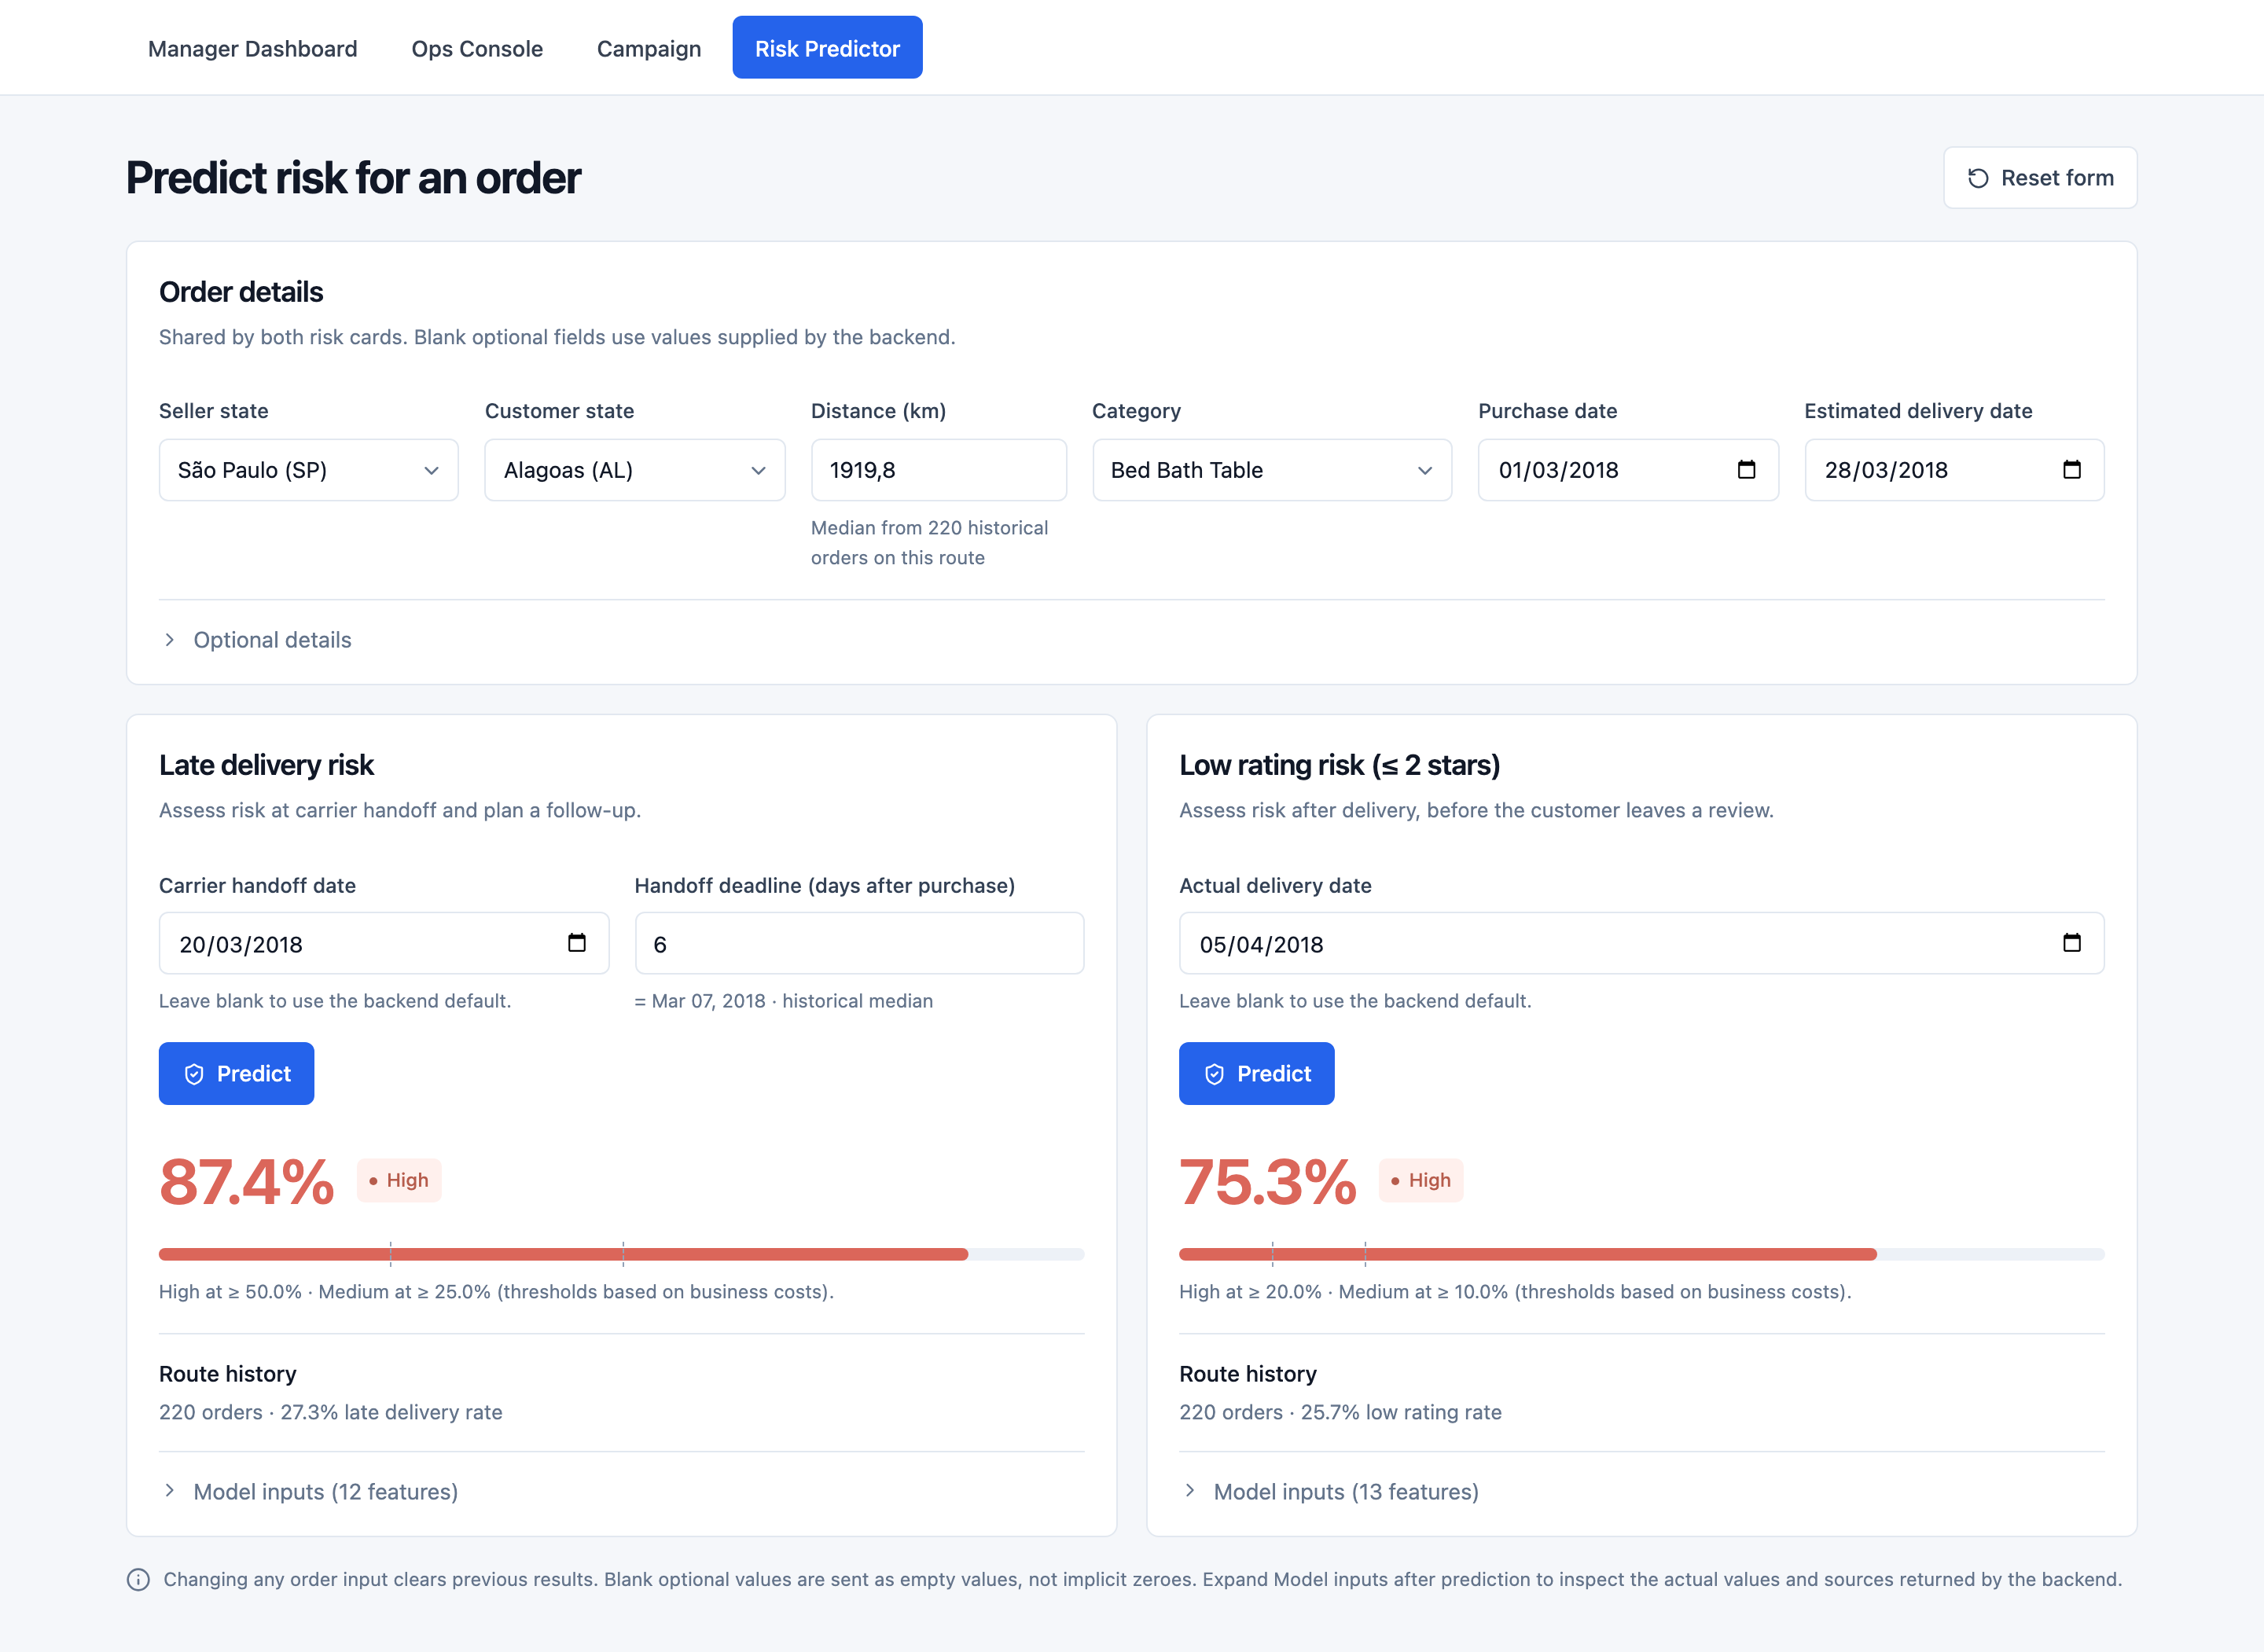
\includegraphics[width=0.85\textwidth]{Picture/ui_predict.png}
\caption{Risk Predictor: đơn giả định tuyến SP $\to$ AL, hẹn giao 27 ngày, người bán bàn giao vào
ngày thứ 19 (rủi ro trễ 87,4\%); nếu giao tới khách trễ 8 ngày thì rủi ro đánh giá thấp 75,3\%}
\label{fig:ui-predict}
\end{figure}

\subsection{Luồng dữ liệu đầu-cuối}
\hspace{1cm}
Hình~\ref{fig:sequence} minh họa luồng xử lý một yêu cầu điển hình từ Manager Dashboard: (1)
người dùng chọn khoảng thời gian trên dashboard; (2) frontend gọi API
\texttt{GET /dashboard/\allowbreak revenue-trend}; (3) backend-api truy vấn \texttt{mv\_revenue\_by\_month\_category}
trên kho dữ liệu; (4) kết quả trả về và được trực quan hóa dưới dạng biểu đồ.

\begin{figure}[H]
\centering
\begin{tikzpicture}[
    actor/.style={draw, rounded corners, fill=black!5, minimum width=2.8cm,
                  minimum height=1.2cm, font=\small, align=center},
    lbl/.style={font=\scriptsize, align=center},
    arr/.style={-{Stealth[length=2mm]}, thick}
]
\node[actor] (fe) at (0,0) {Manager\\Dashboard};
\node[actor] (be) at (7,0) {Backend API\\(BFF)};
\node[actor] (dw) at (14,0) {Kho dữ liệu\\(OLAP view)};

\draw[arr] ([yshift=5pt]fe.east) -- node[above, lbl]{\texttt{GET /dashboard/revenue-trend}\\\texttt{?year=\&category=\&region=}}
    ([yshift=5pt]be.west);
\draw[arr] ([yshift=5pt]be.east) -- node[above, lbl]{\texttt{SELECT ... FROM}\\\texttt{mv\_revenue\_by\_}\\\texttt{month\_category}}
    ([yshift=5pt]dw.west);
\draw[arr] ([yshift=-8pt]dw.west) -- node[below, lbl]{Các dòng kết quả}
    ([yshift=-8pt]be.east);
\draw[arr] ([yshift=-8pt]be.west) -- node[below, lbl]{JSON}
    ([yshift=-8pt]fe.east);
\end{tikzpicture}
\caption{Luồng xử lý một yêu cầu truy vấn doanh thu từ dashboard}
\label{fig:sequence}
\end{figure}

\subsection{Nạp dữ liệu và vận hành thử nghiệm}
\hspace{1cm}
Môi trường demo được khởi tạo theo một trong hai cách: chạy
\texttt{bash scripts/seed\_db.sh} (tạo schema, Extract, Transform,
Load rồi chạy kiểm tra chất lượng, sau đó train mô hình trong container bằng
\texttt{POST /risk/retrain}), hoặc kích hoạt DAG \texttt{staging\_load} trên Airflow để
chuỗi \texttt{staging\_load} $\to$ \texttt{dw\_load} $\to$ \texttt{dss\_batch} tự chạy. Các
dịch vụ backend khởi động bằng \texttt{docker compose up -d}, với Airflow UI tại cổng 8080,
DSS service tại cổng 8001, backend API tại cổng 8000 và PostgreSQL tại cổng 5433; frontend
chạy riêng bằng \texttt{npm run dev} tại cổng 5173.

\textbf{Kết quả vận hành.} Kích hoạt \texttt{staging\_load} trên Airflow, cả ba DAG chạy thành
công nối tiếp nhau, mỗi DAG dưới một phút. Chạy lại không làm thay đổi số dòng (98.666 đơn trong
\texttt{FACT\_ORDER\_FULFILLMENT}, 96.355 phiên bản khách hàng, 38.229 điểm rủi ro) và chỉ số
mô hình giữ nguyên, xác nhận pipeline idempotent và kết quả lặp lại được.

\textbf{Lưu ý về phiên bản thư viện.} File mô hình (\texttt{dss/models/*.pkl}) phải được huấn
luyện bằng cùng phiên bản scikit-learn với container \texttt{dss} (1.9.1); mô hình train trên
máy với phiên bản khác không nạp được trong container. Vì vậy mô hình luôn được huấn luyện lại
bên trong container qua \texttt{POST /risk/retrain} (DAG \texttt{dss\_batch}).

\textbf{Tài liệu trình bày và tái lập kết quả.}
\begin{itemize}
    \item \texttt{dss/notebooks/\allowbreak risk\_models.ipynb}: notebook đi lại từng bước của
          \texttt{dss/risk/\allowbreak train.py} -- đọc dữ liệu từ kho, khám phá dữ liệu, đặc trưng và chống
          leakage, chia theo thời gian, huấn luyện HGB và baseline, ngưỡng theo chi phí, đường
          precision--recall, feature importance, thí nghiệm chấm điểm sớm và drift, what-if. Notebook
          gọi chính các hàm của project và chỉ đọc kho dữ liệu, nên số liệu khớp với hệ thống
          và với Chương~6.
    \item \texttt{report/scripts/make\_figures.py}: vẽ lại các biểu đồ của Chương~6 (tỷ lệ trễ
          theo tháng, đường precision--recall, feature importance) trực tiếp từ kho dữ liệu sau
          mỗi lần huấn luyện lại.
\end{itemize}
